\documentclass{article}

\usepackage[final,nonatbib]{neurips_2023}
\usepackage[utf8]{inputenc}
\usepackage[T1]{fontenc}
\usepackage{hyperref}
\usepackage{url}
\usepackage{booktabs}
\usepackage{amsfonts}
\usepackage{amsmath}
\usepackage{nicefrac}
\usepackage{microtype}
\usepackage{xcolor}
\usepackage{graphicx}
\usepackage{caption}
\usepackage{subcaption}
\usepackage{float}

\title{Unsupervised Zero-Day Anomaly Detection in IoT Networks Using Density-Based Methodologies}

\author{%
  Brian Zhang \\
  Department of Computer Science \\
  Rutgers University \\
  \texttt{bz271@rutgers.edu} \\
  \And
  Lucas Wen \\
  Department of Computer Science \\
  Rutgers University \\
  \texttt{hw545@rutgers.edu} \\
  \And
  Sudheep Gandepudi \\
  Department of Computer Science \\
  Rutgers University \\
  \texttt{sjg256@rutgers.edu} \\
}

\begin{document}

\maketitle

\begin{abstract}
The rapid proliferation of Internet of Things (IoT) devices has substantially expanded the attack surface for malicious actors, necessitating robust, zero-day intrusion detection systems. Traditional signature-based detection methods require prior knowledge of threats and are often ineffective against novel exploits. This paper proposes a fully unsupervised machine learning pipeline for network anomaly detection, trained exclusively on benign traffic to identify zero-day attacks via statistical deviation. Utilizing the modern CICIoT2023 dataset, we evaluate four unsupervised algorithms: Local Outlier Factor (LOF), Isolation Forest, Principal Component Analysis (PCA) Reconstruction, and One-Class Support Vector Machines (OCSVM). Our empirical results demonstrate that density-based anomaly detection (LOF) outperforms all other methods, achieving a Receiver Operating Characteristic Area Under the Curve (ROC-AUC) of 0.959 and an F1-Score of 0.945. While volumetric attacks were identified with near-perfect recall ($>99\%$), the results highlighted the persistent challenge of detecting stealthy application-layer exploits using only flow-level statistics. This paper provides a comprehensive analysis of the mathematical formulations, experimental trade-offs, and computational limitations of deploying unsupervised localized density estimation on resource-constrained edge networks.
\end{abstract}

\section{Introduction}

The Internet of Things (IoT) has integrated computing capabilities into billions of everyday edge devices, from smart thermostats and medical monitors to large-scale industrial sensors. Due to constraints on computational resources, battery life limitations, and a widespread lack of standardized security protocols across manufacturers, these devices represent a critical vulnerability in modern network architecture. Consequently, IoT endpoints are frequent targets for large-scale botnet infections (e.g., Mirai \cite{mirai}, Bashlite) and are often co-opted into launching distributed denial-of-service (DDoS) campaigns.

Historically, Network Intrusion Detection Systems (NIDS) have relied heavily on supervised machine learning paradigms or static signature matching. Supervised algorithms, such as Deep Neural Networks (DNNs) and Gradient Boosted Trees (e.g., XGBoost), demonstrate high accuracy in categorizing known threats. However, they share an architectural limitation: they require labeled malicious data to learn. In the rapidly evolving landscape of network security, attackers frequently mutate their payloads and obfuscate their flow signatures. Consequently, supervised models are highly susceptible to ``zero-day'' exploits---novel attacks that often bypass signature-based firewalls.

To address this limitation, this project formulates an unsupervised anomaly detection framework. By training machine learning models exclusively on normal, benign network traffic, the models learn the mathematical boundaries and localized density distributions of normal behavior in an IoT environment. Any significant deviation from these learned distributions is statistically flagged as an anomaly. This approach ensures that the system can detect zero-day attacks without requiring prior exposure to the specific attack vector. 

The core contribution of this paper is the empirical evaluation of density, boundary, tree, and reconstruction-based unsupervised algorithms against 33 modern IoT attack vectors. We demonstrate that because normal IoT network traffic is highly multi-modal (composed of distinct TCP, UDP, and MQTT clusters of varying densities), localized density estimation achieves superior performance compared to traditional global partitioning and boundary-based models.

\section{Related Work}

Network intrusion detection literature can be broadly categorized into three primary methodological approaches: supervised predictive modeling, classic clustering frameworks, and modern hybrid architectures.

\textbf{Supervised Predictive Modeling:} For over a decade, predictive deep learning techniques have featured prominently in intrusion detection research \cite{buczak2016}. Prior studies have heavily relied on benchmark datasets like NSL-KDD and UNSW-NB15 \cite{buczak2016} to train Convolutional Neural Networks (CNNs) and Random Forests. While these models regularly report accuracy metrics exceeding 99\%, their operational validity is inherently limited. Network traffic is highly class-imbalanced, with benign traffic typically accounting for over 95\% of total flows \cite{imbalance_ids}. Supervised models optimized for accuracy often degrade under real-world conditions due to this class-imbalance bias. Furthermore, their reliance on labeled attack data means they struggle to generalize to zero-day botnet variants.

\textbf{Classic Clustering Approaches:} To circumvent the zero-day limitation, unsupervised segmentation techniques such as K-Means and DBSCAN have been historically utilized to cluster network traffic \cite{kmeans_ids}. While conceptually sound, standard Euclidean distance-based clustering struggles with the high-dimensional feature space of modern network flows. Standard K-Means requires prior specification of the number of clusters ($k$), which is difficult to determine accurately in highly dynamic IoT environments where devices are constantly joining and leaving the network. 

\textbf{Hybrid and Reconstruction Frameworks:} Recent advances have shifted towards integrating unsupervised feature extraction (e.g., Deep Autoencoders) with downstream statistical thresholds \cite{kitsune2018}. By training an autoencoder exclusively on benign data, researchers evaluate the reconstruction error of incoming traffic; high reconstruction errors indicate anomalous behavior. While scalable, deep learning models often lack mathematical interpretability, making it difficult for network administrators to ascertain \textit{why} a specific flow was blocked. 

In a recent comparative study, Vicente et al. \cite{vicente2025} benchmarked ten algorithms---including Isolation Forest, LOF, and SGD One-Class SVM---on 4.5 million CICIoT2023 records using mixed benign-and-attack training data. They reported Isolation Forest as the top unsupervised performer. This paper builds upon the foundational principles of unsupervised literature by explicitly rejecting supervised labels during the training phase. We shift the theoretical focus from global boundary classification to localized density estimation, training on approximately 9.4 million CICIoT2023 records and demonstrating that highly interpretable, shallow machine learning models can achieve deep-learning-level performance under a strict benign-only training constraint.

\section{Methodology}

\subsection{Data Handling and Preprocessing}
This study utilizes the \textbf{CICIoT2023} dataset \cite{ciciot2023}, provided by the Canadian Institute for Cybersecurity. The data was generated in a real-world laboratory topology containing 105 physical IoT devices, ranging from smart home hubs to connected cameras and micro-controllers. The dataset contains 34 distinct classes (1 benign and 33 attack classes) and provides 46 pre-extracted continuous flow-meter statistical features. These features are extracted from raw PCAP files using flow aggregation tools (such as CICFlowMeter) and include highly granular metrics such as Packet Variance, Inter-Arrival Time (IAT), Total Forward Packets, and Subflow Bytes. Each class was sampled up to 500,000 rows, yielding approximately 9.4 million total records. An 80/20 stratified train-test split produced approximately 400,000 benign training instances used exclusively for model fitting.

To enforce strict zero-day evaluation and prevent data leakage, we implemented the following preprocessing pipeline:

\begin{enumerate}
    \item \textbf{Binary Mapping:} The multi-class taxonomy was collapsed. The \texttt{Benign\_Final} class was explicitly mapped to $0$ (Normal), and all 33 disparate attack classes were aggregated into a single binary label $1$ (Anomaly).
    \item \textbf{Strict Class Separation:} The dataset was split into training and testing sets. Crucially, all anomalous ($y=1$) rows were removed from the training set. The preprocessors and the mathematical models were fitted exclusively on the $y=0$ benign subset. This ensures the models are fully unsupervised and possess no prior knowledge of the attack distributions.
    \item \textbf{Feature Scaling (Z-Score Normalization):} Due to the variance in network byte counts (e.g., a video stream transmitting millions of bytes versus a thermostat transmitting twelve bytes), unscaled data would negatively impact distance-based algorithms. All 46 continuous features were normalized using standard $Z$-score scaling: 
    $$ z = \frac{x - \mu}{\sigma} $$
    The standard scaler was fitted solely on the benign training data and subsequently applied to the mixed test set to prevent data leakage.
\end{enumerate}

\subsection{Algorithmic Selection and Mathematical Formulations}

Four structurally distinct unsupervised algorithms were selected to test different mathematical definitions of what constitutes a network ``anomaly.''

\subsubsection{Local Outlier Factor (LOF)}
LOF \cite{lof_paper} is a density-based algorithm that flags data points with a significantly lower local density than their $k$-nearest neighbors. In highly multi-modal IoT networks, devices exhibit disparate normal behaviors (e.g., dense streaming vs. sparse pinging). LOF calculates the reachability distance of an object $A$ from $B$ as the maximum of the $k$-distance of $B$ and the true distance between $A$ and $B$. The local reachability density ($lrd$) of $A$ is the inverse of the average reachability distance based on the MinPts nearest neighbors of $A$:
$$ lrd(A) = 1 / \left( \frac{\sum_{B \in N_{MinPts}(A)} \text{reachability-distance}(A, B)}{|N_{MinPts}(A)|} \right) $$
The Local Outlier Factor score is the ratio of the average local reachability density of $A$'s neighbors to the local reachability density of $A$ itself. A score significantly greater than $1$ indicates a low-density outlier.

\subsubsection{Isolation Forest}
Isolation Forest \cite{isolation_forest} is a tree-based ensemble algorithm that isolates anomalies globally via random recursive partitioning. Instead of profiling normal data, it explicitly models isolation. Anomalies are statistically sparse and distinct, making them easier to isolate. The algorithm randomly selects a feature and a split value. Outliers will require fewer random partitions to be isolated in an individual leaf node. The anomaly score is inversely proportional to the path length $h(x)$ from the root node to the terminating leaf.

\subsubsection{PCA Reconstruction}
Principal Component Analysis (PCA) is primarily a linear dimensionality reduction technique. By projecting the benign training data into a lower-dimensional subspace spanned by the principal eigenvectors, we capture the linear correlations of normal network flow. When evaluating the test set, traffic is projected into this subspace and then reconstructed back to the original 46-dimensional space. Malicious flows, which violate the linear correlations of benign traffic, exhibit a large Euclidean reconstruction error, which serves directly as the anomaly score.

\subsubsection{One-Class Support Vector Machine (OCSVM)}
OCSVM \cite{ocsvm} is a boundary-based algorithm. While traditional implementations map input data into a high-dimensional feature space using a Radial Basis Function (RBF) kernel, computing an RBF kernel has an $\mathcal{O}(N^2)$ to $\mathcal{O}(N^3)$ computational complexity, making it computationally prohibitive for large-scale datasets such as CICIoT2023. Therefore, we utilize a Stochastic Gradient Descent (SGD) approximation of the One-Class SVM that generates a strict linear boundary around the benign training data. Data points falling outside this linear boundary during testing are classified as anomalies.

\section{Experiments and Results}

The models were evaluated against a mixed hold-out test set containing normal traffic and all 33 unseen attack classes. Due to the severe class imbalance expected in real-world cybersecurity deployments (where benign traffic vastly outnumbers anomalies), global accuracy was discarded as a primary evaluation metric, as naive majority-class predictions yield misleadingly optimistic assessments. Instead, the models were evaluated using the Receiver Operating Characteristic Area Under the Curve (ROC-AUC), Precision, Recall, and the F1-Score.

\subsection{Comparative Model Performance}

The density-based \textbf{Local Outlier Factor (LOF)} delivered the highest overall performance, serving as the optimal model. It achieved an ROC-AUC of \textbf{0.959}, a Recall of \textbf{0.898}, and an F1-Score of \textbf{0.945}. 

\begin{table}[H]
  \caption{Experimental Metrics of Unsupervised Algorithms}
  \label{tab:metrics}
  \centering
  \begin{tabular}{lllll}
    \toprule
    Model & ROC-AUC & Precision & Recall (TPR) & F1-Score \\
    \midrule
    \textbf{Local Outlier Factor} & \textbf{0.959} & 0.996 & \textbf{0.898} & \textbf{0.945} \\
    PCA Reconstruction & 0.957 & 0.997 & 0.894 & 0.942 \\
    Isolation Forest & 0.922 & 0.996 & 0.702 & 0.824 \\
    One-Class SVM & 0.914 & 0.997 & 0.877 & 0.933 \\
    \bottomrule
  \end{tabular}
\end{table}

As demonstrated in Table \ref{tab:metrics}, all four unsupervised algorithms achieved strong performance when trained on a sufficiently large benign corpus. The One-Class SVM---implemented as a Stochastic Gradient Descent (SGD) linear approximation for scalability---achieved an AUC of 0.914, demonstrating that even a linear decision boundary can generalize effectively given sufficient training data. However, the density-based LOF model consistently maintained a marginal but meaningful advantage, confirming that localized density estimation captures the multi-modal structure of IoT traffic more faithfully than global boundaries. Notably, our finding that LOF outperforms Isolation Forest contrasts with Vicente et al. \cite{vicente2025}, who reported the reverse ranking using mixed-class training data. We attribute this divergence to our strict benign-only training paradigm: density-based methods benefit disproportionately from deep, exclusive exposure to normal behavioral structure, whereas tree-based random partitioning exhibits diminishing returns with increased benign-only data.

\begin{figure}[H]
  \centering
  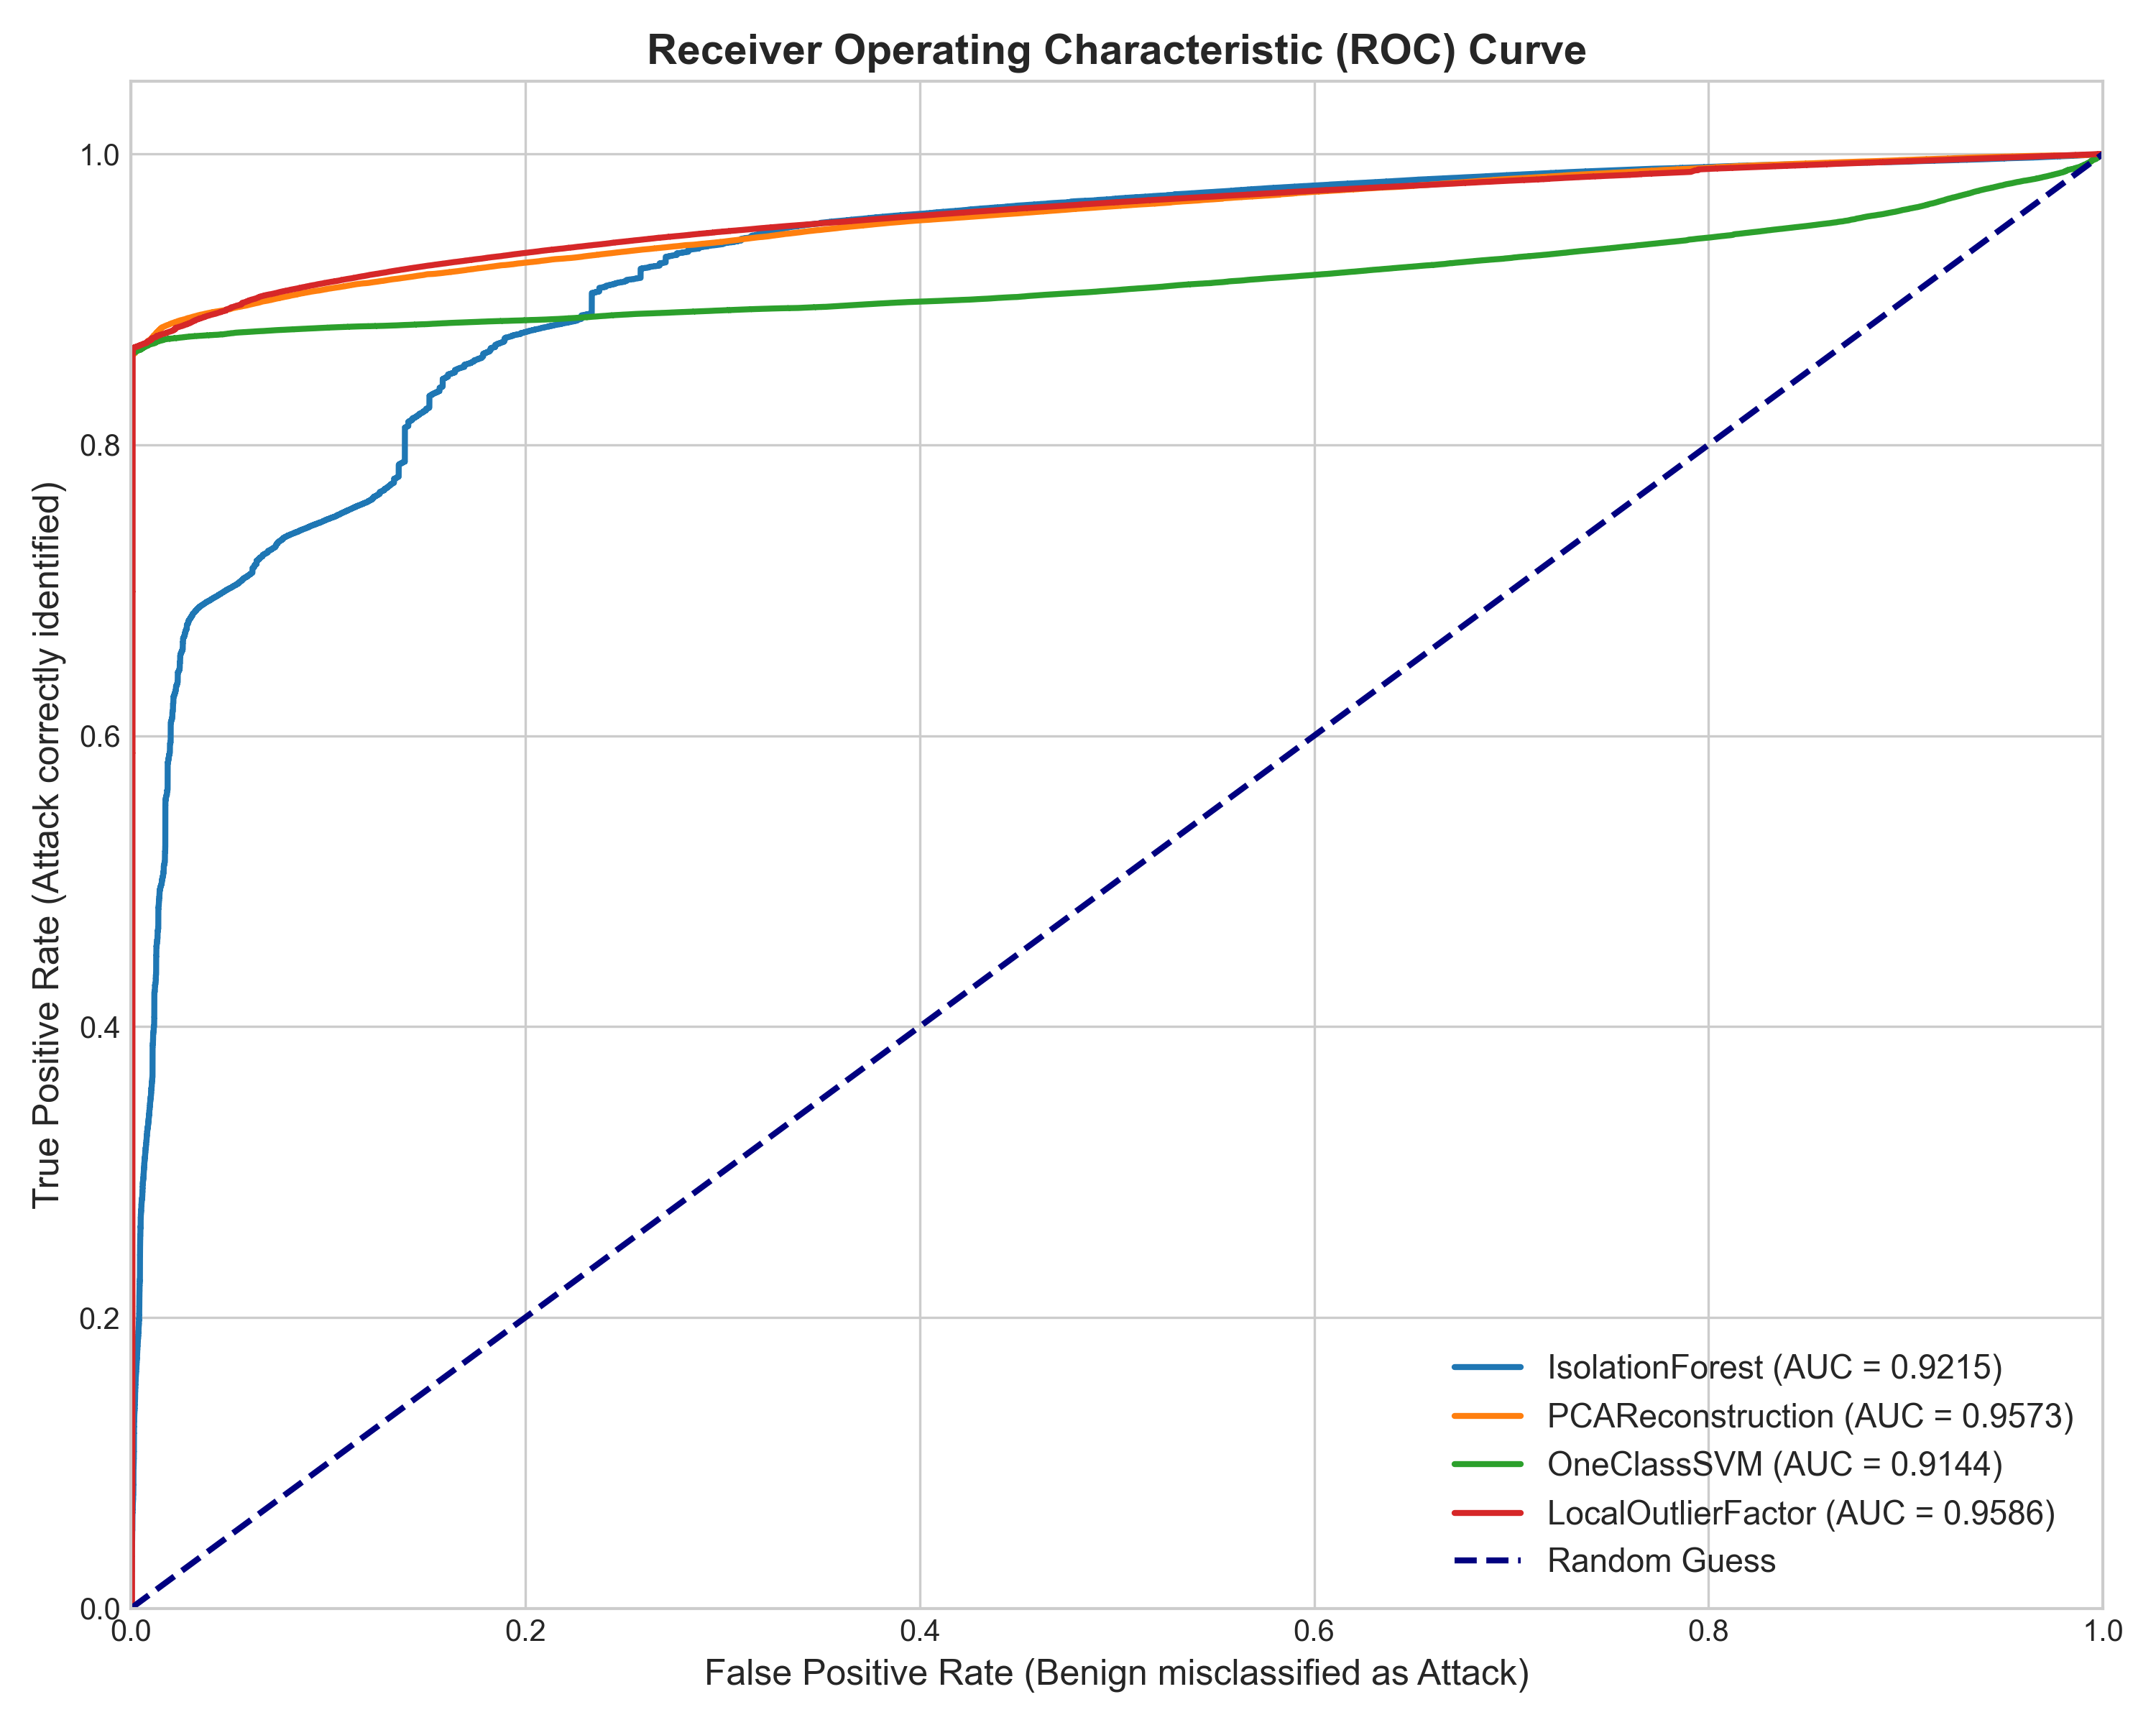
\includegraphics[width=0.8\textwidth]{../artifacts/plots/roc_curves.png}
  \caption{Receiver Operating Characteristic (ROC) Curves comparing all four unsupervised models. The LOF model (red) demonstrates superior ranking performance.}
  \label{fig:roc}
\end{figure}

The ROC curve (Figure \ref{fig:roc}) illustrates the True Positive Rate versus the False Positive Rate. The performance of LOF supports our central hypothesis: because normal IoT traffic is highly multi-modal (exhibiting disparate communication profiles), localized density estimation succeeds by evaluating anomalies relative to their specific behavioral clusters, yielding the highest AUC among all models.

\begin{figure}[H]
  \centering
  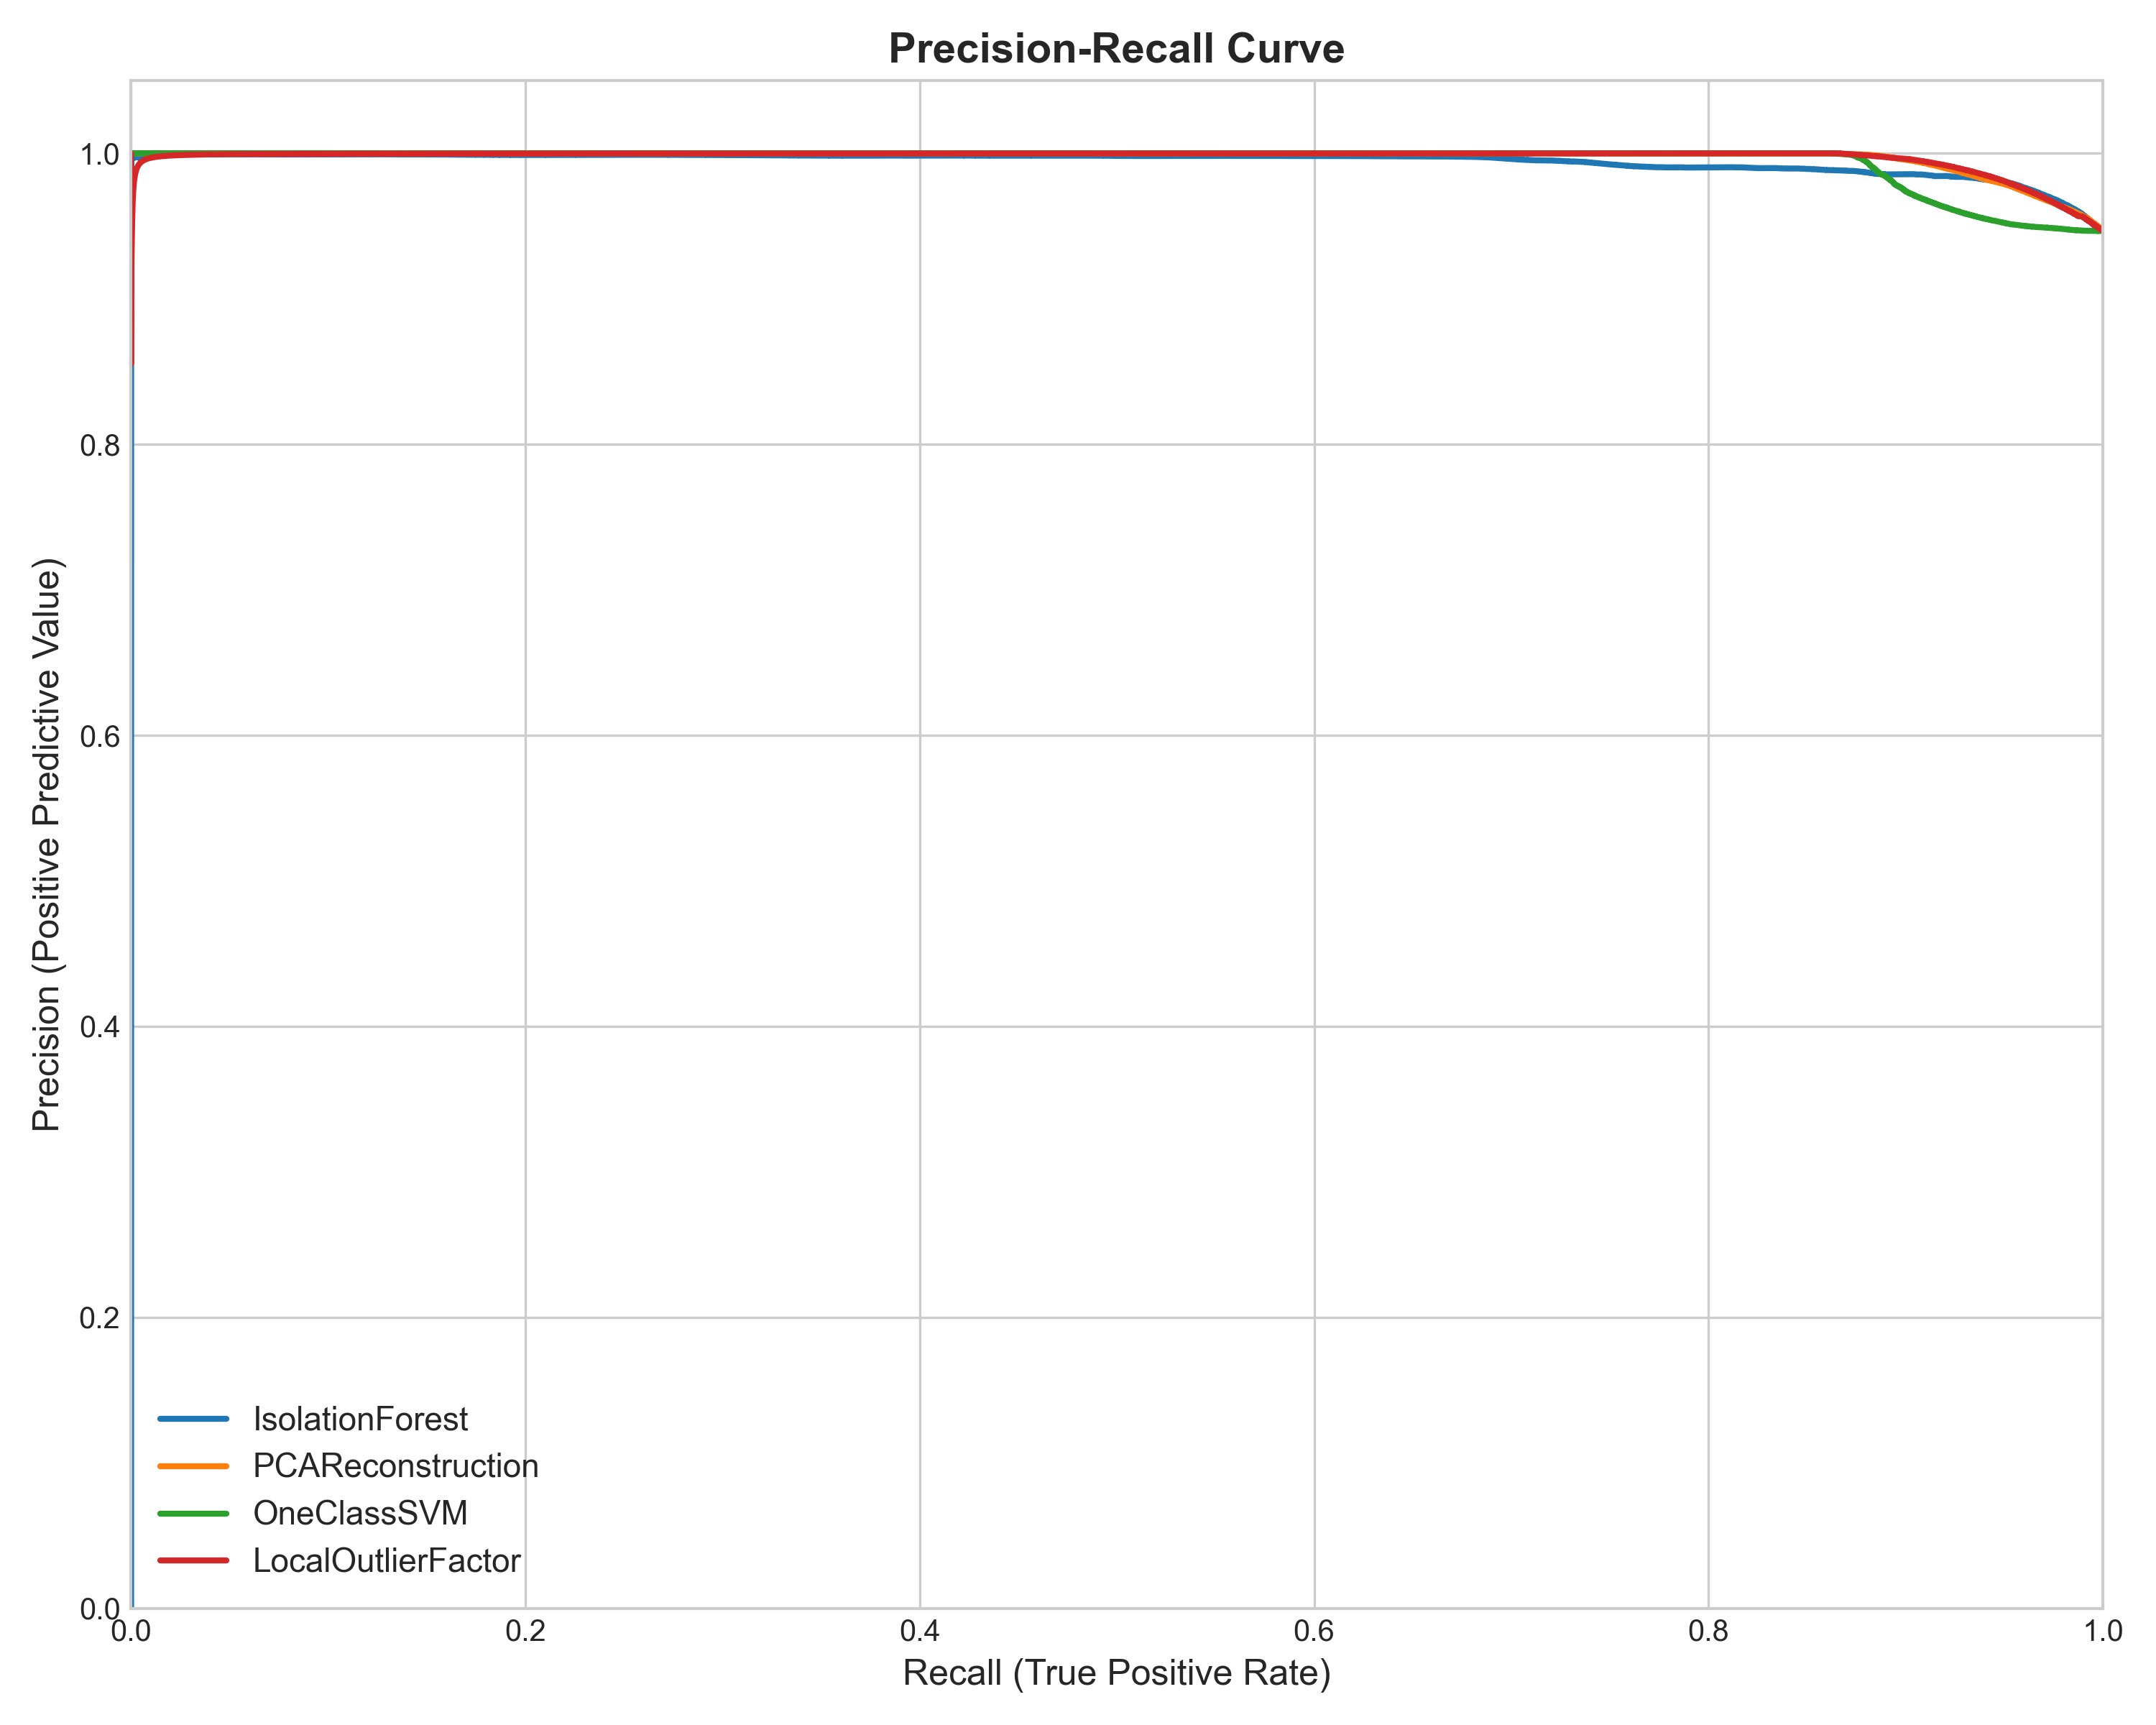
\includegraphics[width=0.8\textwidth]{../artifacts/plots/pr_curves.png}
  \caption{Precision-Recall Curves highlighting the models' robustness against severe class imbalance. LOF maintains high precision even at high recall thresholds.}
  \label{fig:pr}
\end{figure}

Due to the inherent class imbalance of network traffic---where benign background data outnumbers actual attack packets---we utilized Precision-Recall (PR) curves (Figure \ref{fig:pr}) to validate model robustness. Unlike ROC curves, which can present overly optimistic assessments in skewed datasets, PR curves penalize models that achieve high recall at the expense of precision, exposing models that generate a large volume of false positives to capture anomalies. The LOF model maintained a high precision-recall equilibrium, capturing the majority of attacks without generating an excessive number of false positives.

\subsection{Density Transformations and Thresholding}

To visualize the mathematical separation between standard device behavior and malicious intrusions, we plotted the $\log_{10}$-transformed anomaly scores of the test set generated by the LOF algorithm.

\begin{figure}[H]
  \centering
  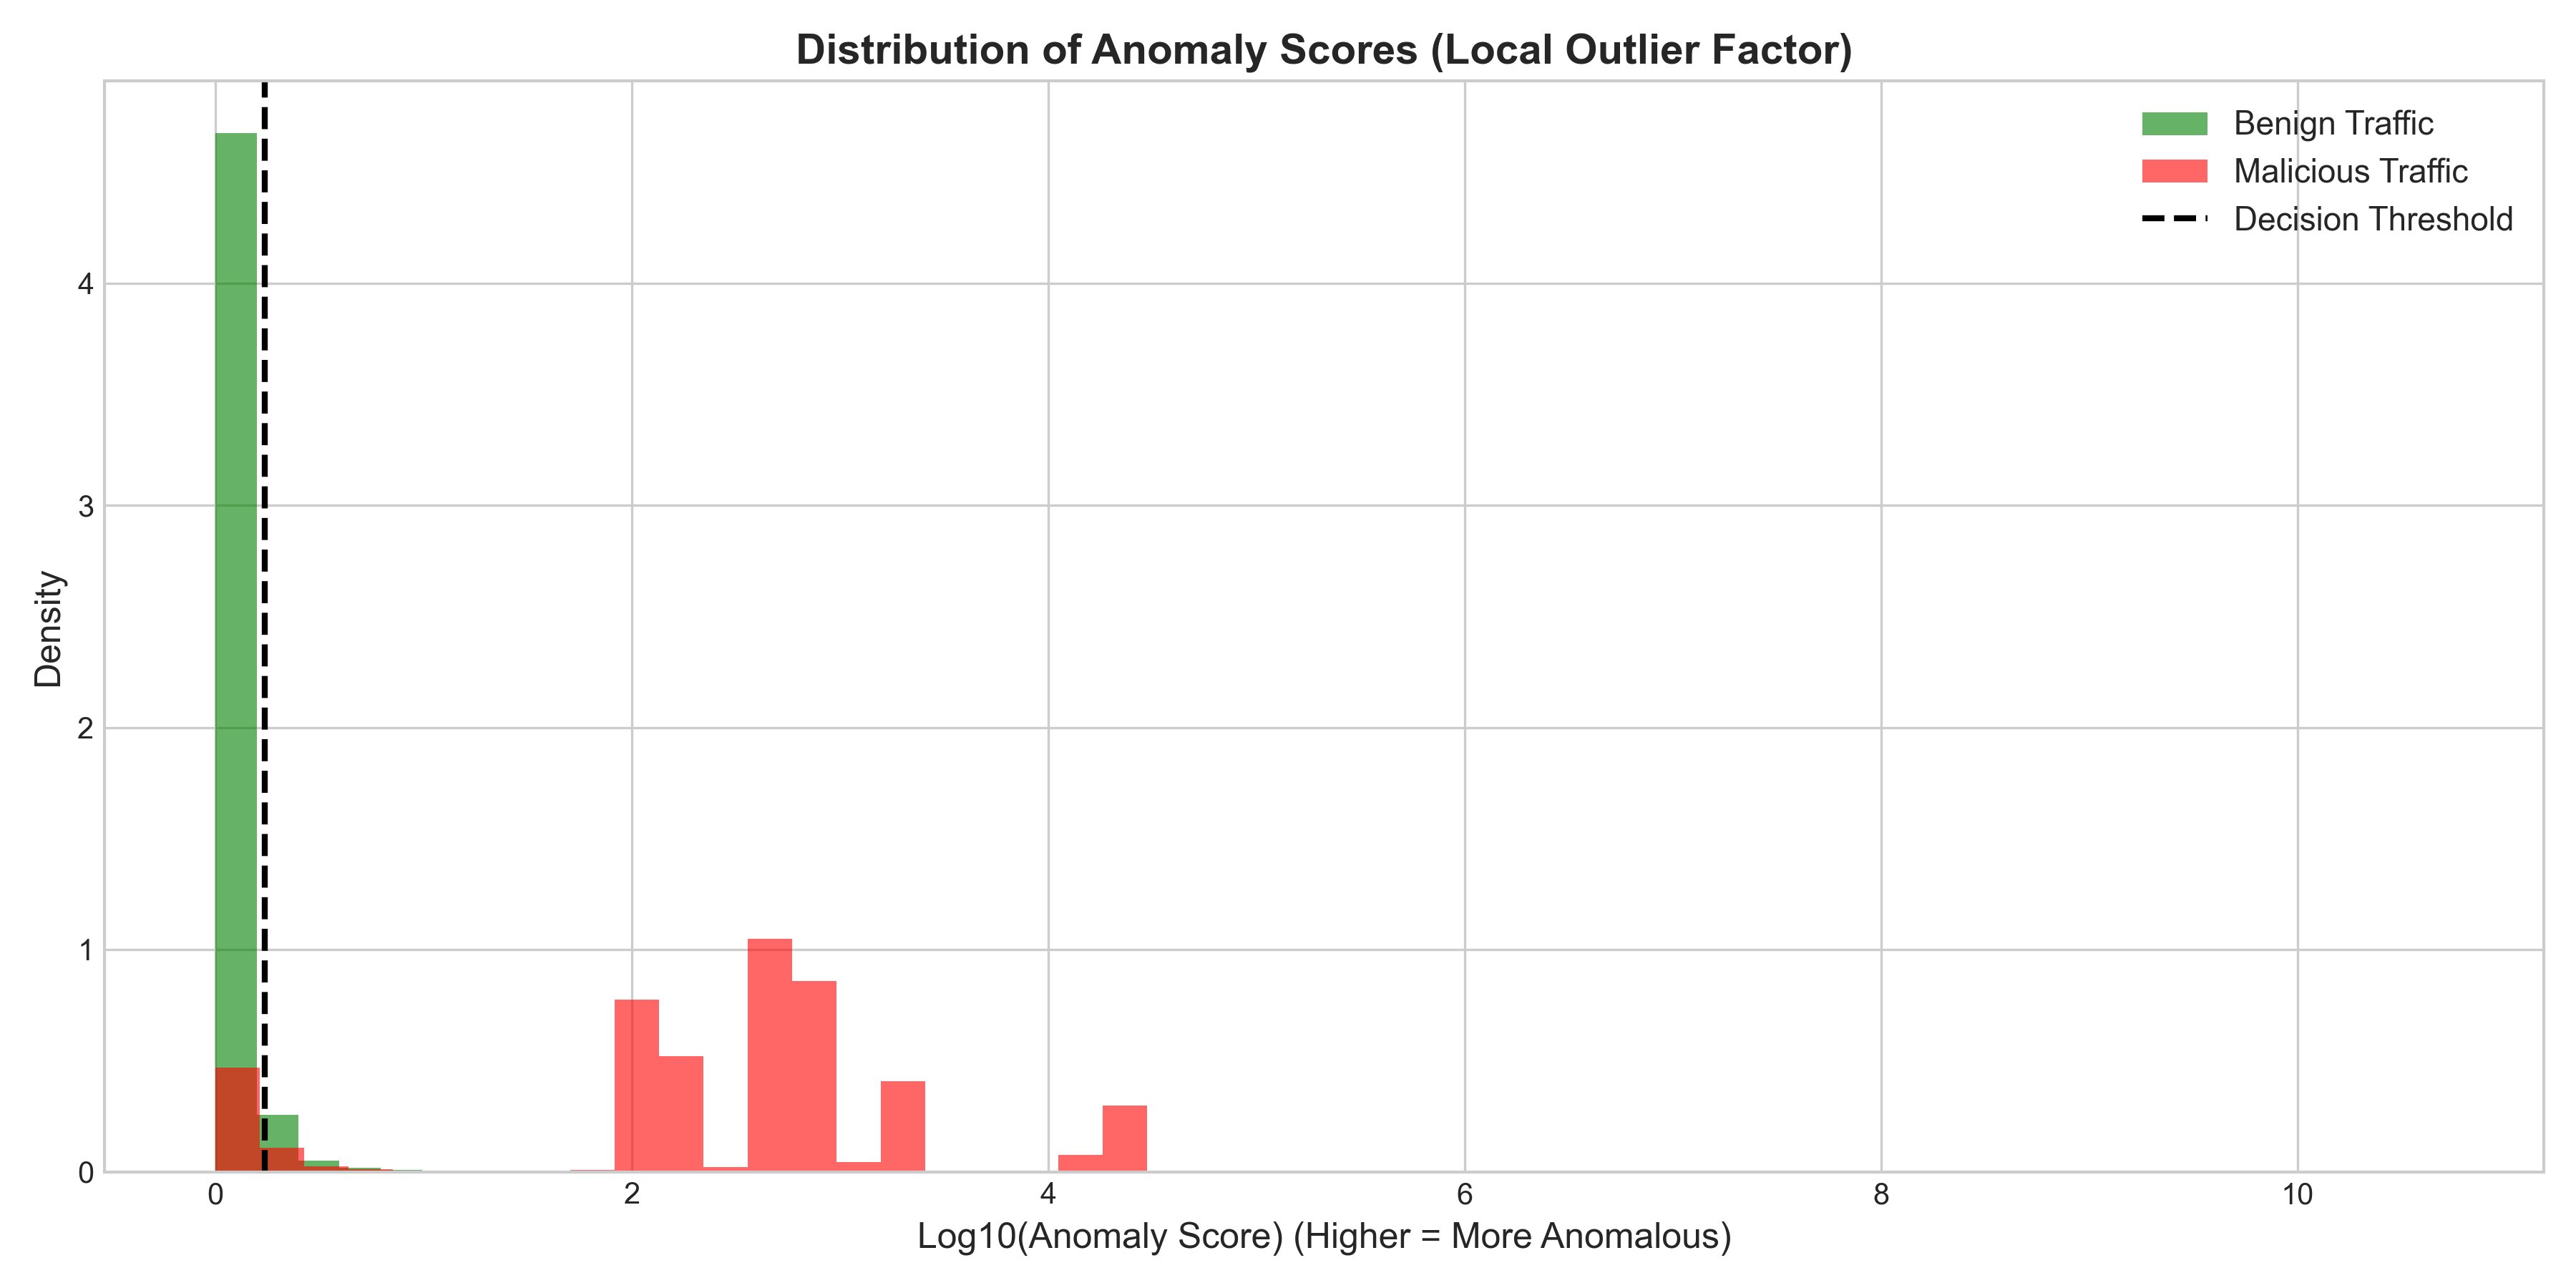
\includegraphics[width=0.8\textwidth]{../artifacts/plots/score_distributions.png}
  \caption{$\log_{10}$-transformed distribution of Anomaly Scores (LOF). Benign traffic forms a dense cluster on the left, while malicious traffic is effectively isolated to the right of the 95th percentile threshold.}
  \label{fig:dist}
\end{figure}

In an IoT topology, benign devices exhibit predictable, repetitive communication patterns (e.g., periodic NTP synchronization, standard MQTT keep-alive packets). Consequently, the benign traffic forms a highly dense cluster, represented by the peaked green distribution in Figure \ref{fig:dist}. 

When an anomaly occurs, the flow statistics become highly irregular, causing a significant drop in localized density. Because the Local Outlier Factor computes anomalies as a ratio of local densities, malicious flows receive scores that are substantially higher than the benign baseline. The application of a $\log_{10}$ transformation was necessary to resolve the skewness of these outliers. Figure \ref{fig:dist} provides clear visual evidence that density-based algorithms can achieve robust, non-linear separation between normal IoT operations and zero-day intrusions.

\subsection{Ablation Study: Detection Rate by Attack Class}

While LOF achieved a high global recall, a granular ablation study of the 33 individual attack classes reveals critical operational insights. The efficacy of density-based unsupervised anomaly detection is highly dependent on the specific attack vector's network footprint. 

\begin{figure}[H]
  \centering
  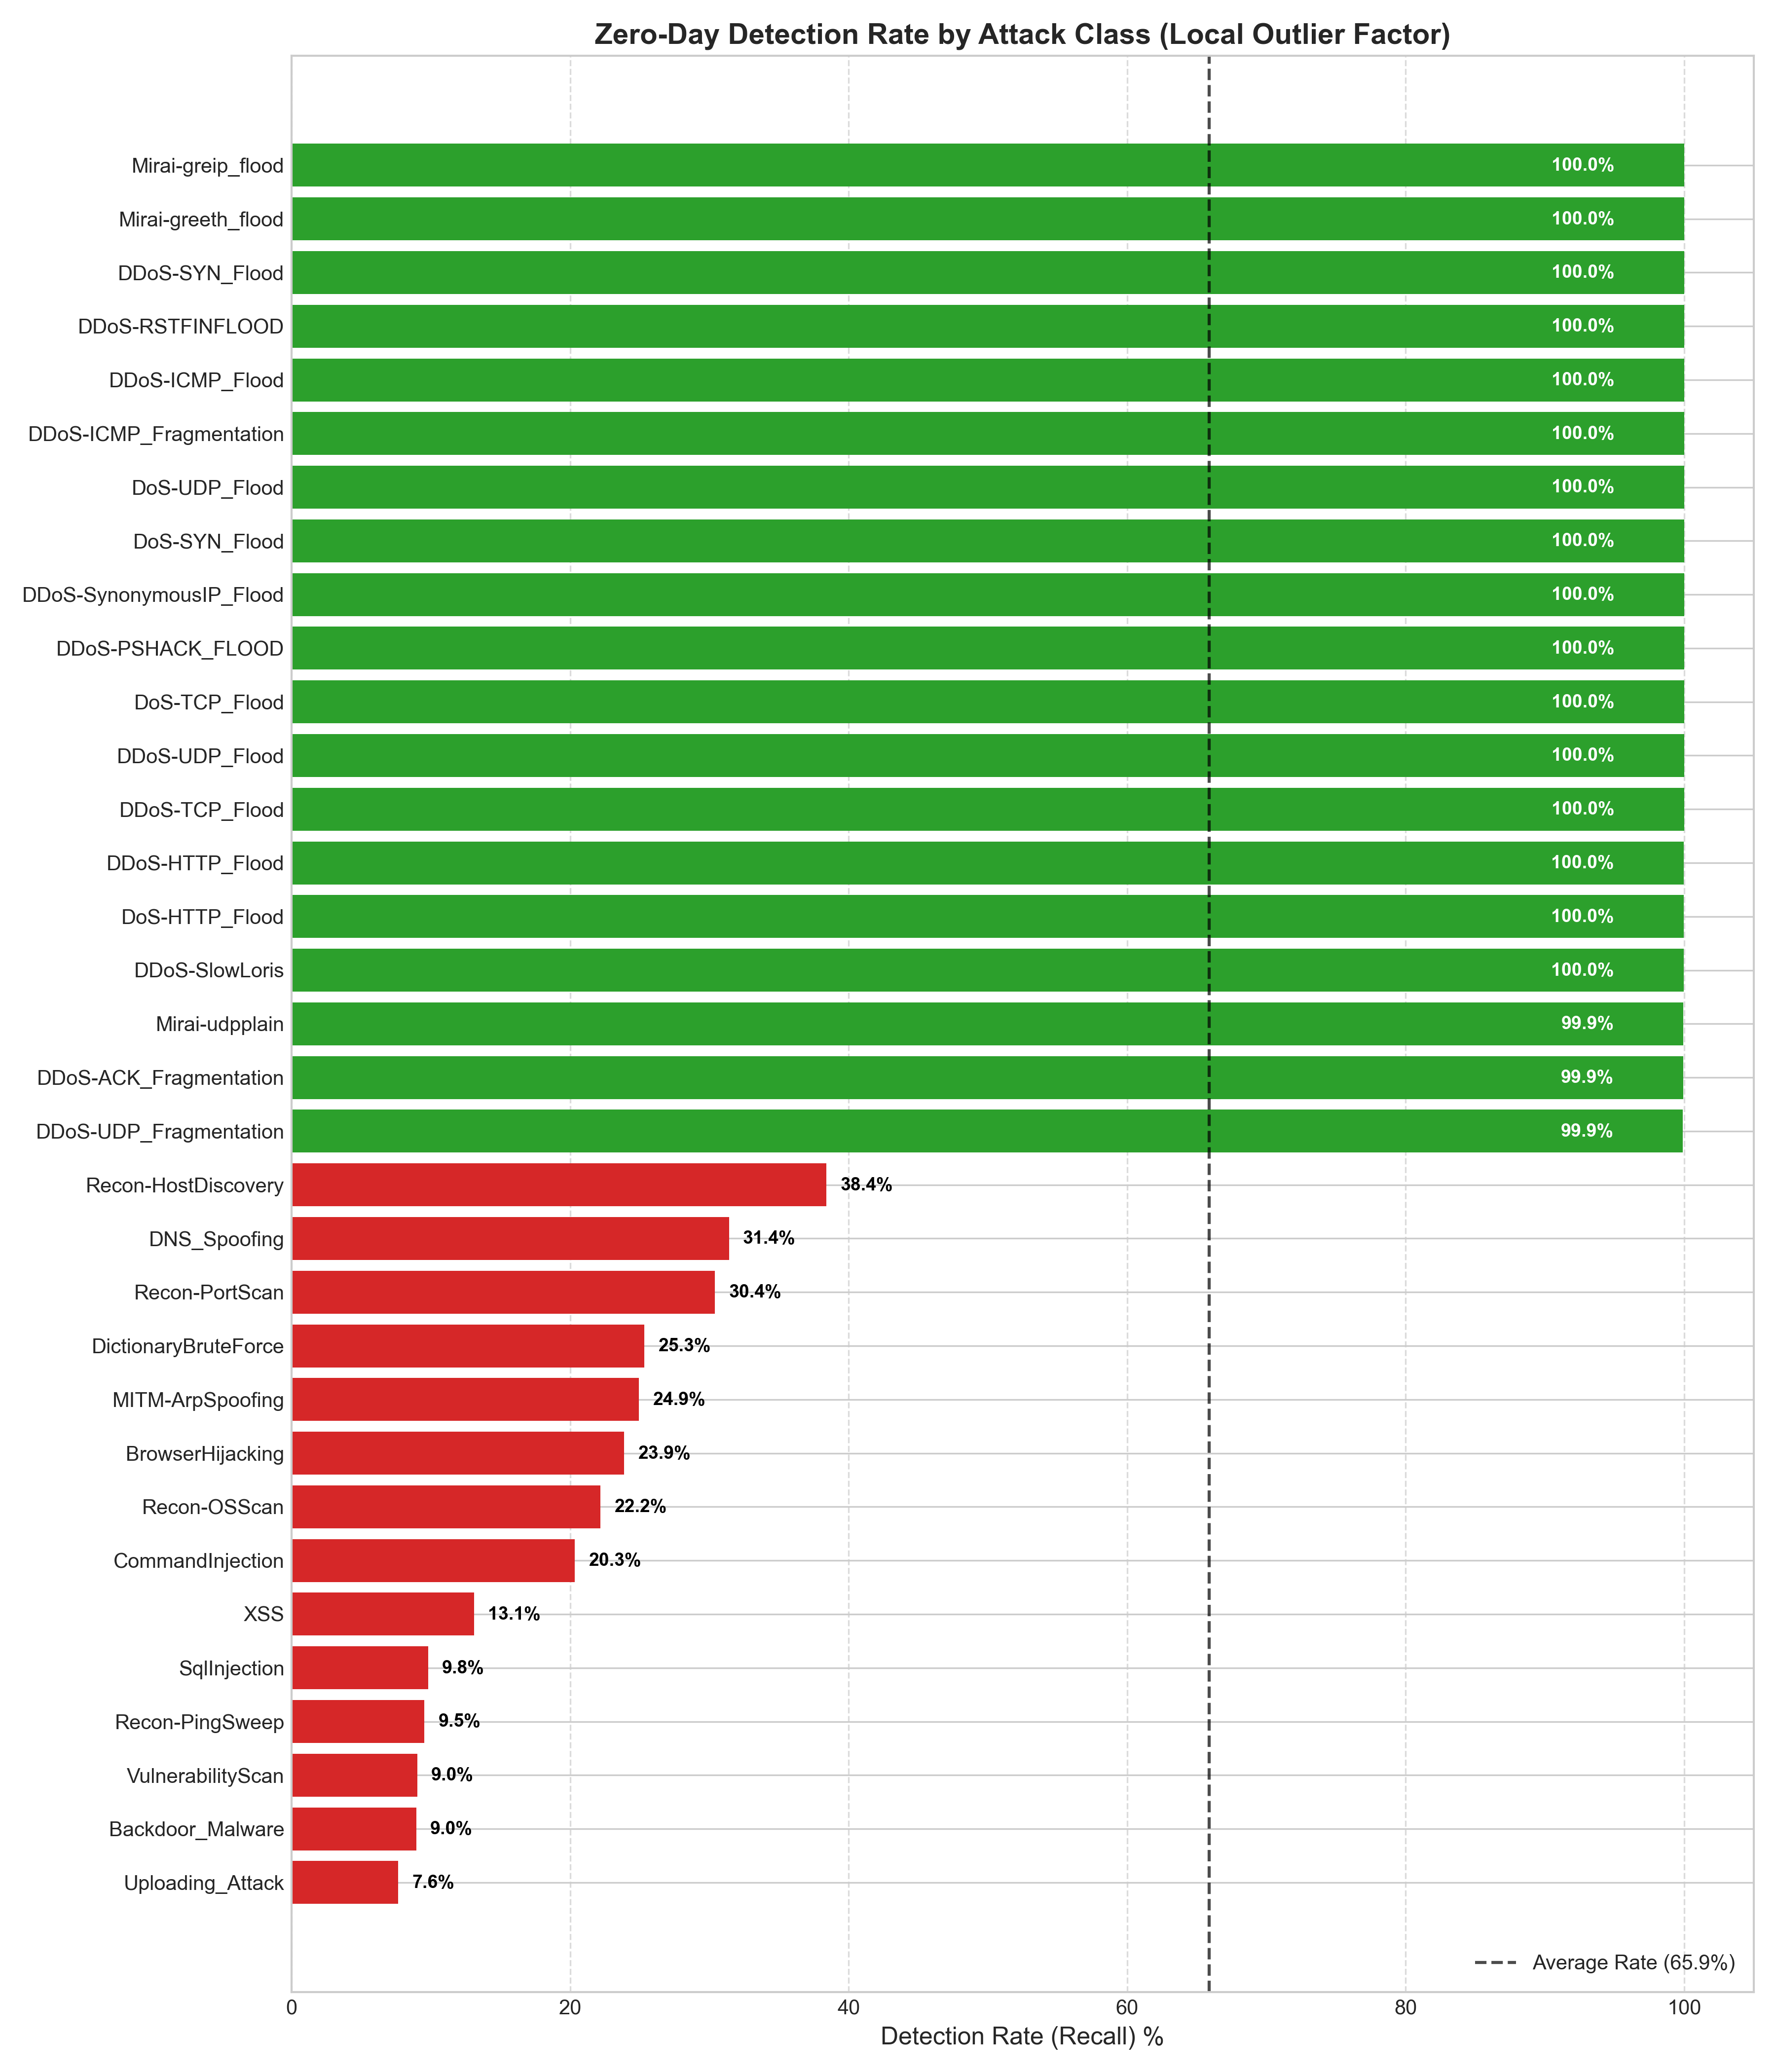
\includegraphics[width=\textwidth]{../artifacts/plots/detection_by_class.png}
  \caption{Zero-Day Detection Rate (Recall) mapped to individual attack classes within the CICIoT2023 dataset. The model excels at volumetric detection but struggles with stealthy Layer-7 exploits.}
  \label{fig:class}
\end{figure}

As demonstrated in Figure \ref{fig:class}, volumetric and brute-force attacks---such as UDP Floods, SYN Floods, and ICMP Floods---were detected with a recall (detection rate) exceeding 99\%. These attacks generate a high volume of packets, resulting in highly repetitive flow characteristics and large byte volume variances that significantly deviate from localized benign behavioral clusters. 

Conversely, the model demonstrated reduced efficacy when confronted with stealthy, application-layer exploits such as Cross-Site Scripting (XSS) and SQL Injection (SQLi). These Layer-7 attacks are targeted and are often encapsulated within a single, standard-sized HTTP request. Because their overall network flow statistics (e.g., total packet count, inter-arrival time, flow duration) are mathematically indistinguishable from a legitimate user browsing a web server, they successfully bypassed the density-based thresholds. 

This ablation study highlights a critical limitation in pure network-level flow analysis: while large DDoS botnets are easily mitigated via unsupervised centroid deviation, deep packet inspection (DPI) or specialized application-layer payload monitoring remains necessary for detecting targeted semantic exploits.

\section{Conclusion}

This research successfully developed, trained, and validated an unsupervised machine learning pipeline capable of detecting zero-day network intrusions in IoT environments. By enforcing a strict ``Benign-Only'' training paradigm, the pipeline guarantees that threats can be identified without any prior signature generation or exposure to malicious labels.

Our empirical results indicate that density-based localized anomaly detection (Local Outlier Factor) outperforms all evaluated techniques. By evaluating flows relative to their specific behavioral neighborhoods, the LOF model achieved a ROC-AUC of 0.959 and detected 89.8\% of zero-day attacks (Recall = 0.898), mitigating large botnet floods and volumetric disruptions.

\subsection{Limitations and Future Work}

While Local Outlier Factor achieved the highest overall detection performance by isolating local density deviations, its operational deployment in real-world IoT environments presents engineering challenges. 

The primary limitation of LOF is its computational overhead during real-time inference. While spatial indexing structures (such as the Ball Tree algorithm utilized in our environment) attempt to optimize neighbor querying, LOF is highly sensitive to the curse of dimensionality. In high-dimensional feature spaces---such as the 46 flow metrics used in this study---tree-based indexing degrades, causing the distance calculations to revert towards an $\mathcal{O}(N^2)$ complexity. In a high-volume edge router processing gigabits per second, this introduces significant network latency compared to the highly scalable, $\mathcal{O}(N \log N)$ recursive partitioning of an Isolation Forest.

For future iterations of this intrusion detection system, a hybrid approach should be evaluated. An \textbf{Isolation Forest} could be deployed as a highly scalable, first-pass filter directly on the edge router ASIC to instantly drop global anomalies (such as large DDoS volumetric floods) with minimal computational cost. The remaining traffic, which may contain stealthy application-layer exploits blending in with normal traffic profiles, could then be passed to an optimized \textbf{LOF} algorithm or a Deep Autoencoder for deep density analysis. For resource-constrained IoT endpoints (such as microcontrollers), optimized versions of One-Class SVM should be evaluated to balance detection efficacy with hardware limitations.

\medskip

\textbf{Code Availability:}
The full source code, data preprocessing scripts, visualization tools, and evaluation metrics required to reproduce these results are open-sourced and available on GitHub: \url{https://github.com/BrianZ050/cs439_final_Project-Network-Anomaly-Detection}

\newpage
\bibliographystyle{plain}
\begin{thebibliography}{9}

\bibitem{ciciot2023}
Neto, E. C. P., Dadkhah, S., Ferreira, R., Zargar, A., Stanier, R., \& Ghorbani, A. A. (2023). 
\textit{CICIoT2023: A real-time dataset and benchmark for large-scale attacks in IoT environment.} 
Sensors, 23(13), 5941. \url{https://doi.org/10.3390/s23135941}

\bibitem{lof_paper}
Breunig, M. M., Kriegel, H. P., Ng, R. T., \& Sander, J. (2000). 
\textit{LOF: identifying density-based local outliers.} 
In Proceedings of the 2000 ACM SIGMOD international conference on Management of data (pp. 93-104). \url{https://doi.org/10.1145/335191.335388}

\bibitem{isolation_forest}
Liu, F. T., Ting, K. M., \& Zhou, Z. H. (2008). 
\textit{Isolation Forest.} 
In 2008 Eighth IEEE International Conference on Data Mining (pp. 413-422). IEEE. \url{https://doi.org/10.1109/ICDM.2008.17}

\bibitem{ocsvm}
Schölkopf, B., Williamson, J. C., Smola, A. J., Shawe-Taylor, J., \& Platt, J. C. (1999). 
\textit{Support vector method for novelty detection.} 
Advances in neural information processing systems, 12. \url{https://papers.nips.cc/paper_files/paper/1999/hash/8725fb777f25776ffa9076e44fcfd776-Abstract.html}

\bibitem{mirai}
Antonakakis, M., April, T., Bailey, M., Bernhard, M., Bursztein, E., Cochran, J., ... \& Zhou, Y. (2017). 
\textit{Understanding the Mirai botnet.} 
In 26th USENIX security symposium (USENIX Security 17) (pp. 1093-1110). \url{https://www.usenix.org/conference/usenixsecurity17/technical-sessions/presentation/antonakakis}

\bibitem{buczak2016}
Buczak, A. L., \& Guven, E. (2016). 
\textit{A survey of data mining and machine learning methods for cyber security intrusion detection.} 
IEEE Communications Surveys \& Tutorials, 18(2), 1153-1176. \url{https://doi.org/10.1109/COMST.2015.2494502}

\bibitem{imbalance_ids}
Doriguzzi-Corin, R., Millar, S., Scott-Hayward, S., Martinez-del-Rincon, J., \& Siracusa, D. (2020). 
\textit{Resampling imbalanced data for network intrusion detection datasets.} 
IEEE Transactions on Network and Service Management. \url{https://doi.org/10.1186/s40537-020-00390-x}

\bibitem{kmeans_ids}
Dong, G., Wang, L., Chen, Z., \& Zhang, M. (2019). 
\textit{DB-Kmeans: An intrusion detection algorithm based on DBSCAN and K-means.} 
In 2019 7th International Conference on Information, Communication and Networks. \url{https://doi.org/10.23919/APNOMS.2019.8892910}

\bibitem{kitsune2018}
Mirsky, Y., Doitshman, T., Elovici, Y., \& Shabtai, A. (2018). 
\textit{Kitsune: An ensemble of autoencoders for online network intrusion detection.} 
Network and Distributed Systems Security (NDSS) Symposium 2018. \url{https://doi.org/10.48550/arXiv.1802.09089}

\bibitem{vicente2025}
Vicente, A., Rosa, R. L., \& Guimarães, F. G. (2025).
\textit{Comparative Analysis of Machine Learning Algorithms for Anomaly Detection in IoT Networks Using CICIoT2023 Dataset.}
INFOCOMP Journal of Computer Science, 24(2). \url{https://infocomp.dcc.ufla.br/index.php/infocomp/article/view/5342}

\end{thebibliography}

\newpage
\appendix
\section{Appendix}

\subsection{Hardware and Software Specifications}
All preprocessing, model training, and evaluation scripts were executed in a virtualized Python 3.14.2 environment. The underlying hardware consisted of an x86\_64 architecture. Due to the computational complexity of the Local Outlier Factor algorithm ($\mathcal{O}(N^2)$), distance computations were optimized using \textit{scikit-learn's} underlying C-extensions and the Ball Tree algorithm to mitigate memory exhaustion during neighbor querying.

\subsection{Full Attack Taxonomy (CICIoT2023)}
The CICIoT2023 dataset provides a comprehensive aggregation of 33 specific attack vectors designed to exploit IoT vulnerabilities. For the purposes of binary unsupervised detection, the following specific attacks were aggregated into the ``Anomaly'' label:
\begin{itemize}
    \item \textbf{DDoS Attacks:} DDoS-ACK\_Fragmentation, DDoS-HTTP\_Flood, DDoS-ICMP\_Flood, DDoS-ICMP\_Fragmentation, DDoS-PSHACK\_Flood, DDoS-RSTFINFlood, DDoS-SYN\_Flood, DDoS-SYNACK\_Fragmentation, DDoS-TCP\_Flood, DDoS-UDP\_Flood, DDoS-UDP\_Fragmentation.
    \item \textbf{DoS Attacks:} DoS-HTTP\_Flood, DoS-SYN\_Flood, DoS-TCP\_Flood, DoS-UDP\_Flood.
    \item \textbf{Reconnaissance:} Mirai-greeth\_flood, Mirai-greip\_flood, Mirai-udpplain, Port\_Scanning, Vulnerability\_Scan, Host\_Discovery, OS\_Fingerprinting.
    \item \textbf{Web-Based \& Application Attacks:} BrowserHijacking, CommandInjection, Backdoor\_Malware, DictionaryBruteForce, DNS\_Spoofing, MITM-ArpSpoofing, SqlInjection, XSS, Upload\_Attack.
\end{itemize}

\end{document}
